\documentclass{llncs}
\pagestyle{plain}
\usepackage[show]{ed}
\usepackage[utf8]{inputenc}
\usepackage{xspace}
\usepackage{amsfonts}
\usepackage{listings}
\usepackage{wrapfig}
\usepackage[style=alphabetic,backend=bibtex,isbn=false]{biblatex}
\usepackage{tikzinput}
\usetikzlibrary{backgrounds,shadows,shapes,fit}
\usetikzlibrary{decorations.pathmorphing}

\addbibresource{../../lib/kbibs/kwarcpubs.bib}
\addbibresource{../../lib/kbibs/extpubs.bib}
\addbibresource{../../lib/kbibs/kwarccrossrefs.bib}
\addbibresource{../../lib/kbibs/extcrossrefs.bib}
\addbibresource{rest.bib}% add bibs here!
\renewbibmacro*{event+venue+date}{}
\renewbibmacro*{doi+eprint+url}{%
  \iftoggle{bbx:doi}
    {\printfield{doi}\iffieldundef{doi}{}{\clearfield{url}}}
    {}%
  \newunit\newblock
  \iftoggle{bbx:eprint}
    {\usebibmacro{eprint}}
    {}%
  \newunit\newblock
  \iftoggle{bbx:url}
    {\usebibmacro{url+urldate}}
    {}}
  
\usepackage{hyperref}
\title{REGULAR-T1: Knowledge-Based Interoperability for Mathematical Software Systems}
\author{
Michael Kohlhase\inst{1} 
Dennis M\"uller\inst{1} 
Markus Pfeiffer\inst{3} 
Florian Rabe\inst{2} 
Nicolas~M.~Thiéry\inst{4} 
Victor Vasilyev\inst{3} 
Tom Wiesing\inst{1}
}

\institute{
   FAU Erlangen-N\"urnberg
   \and Jacobs University Bremen
   \and University of St~Andrews 
   \and Universit\'e Paris-Sud
}
\begin{document}
\maketitle
\begin{abstract}
  There is a large, open-source ecosystem of mathematical software systems that collect and
  classify, compute with, prove statements about, and visualize mathematical objects and
  models. Individually, these systems are optimized for particular domains and
  functionalities and together they cover many, but no system covers all needs of
  practical and theoretical mathematics. System integrations exist, but are ad-hoc and
  have scalability and maintainability issues. In particular, there is not yet an
  interoperability layer that combines them into a virtual research environment (VRE) for
  mathematics.
  
  The OpenDreamKit project, which aims at a mathematical VRE toolkit, proposes the
  Math-in-the-Middle (MitM) paradigm, an interoperability framework based on a flexiformal
  representation of mathematical knowledge and aligns this with system-generated interface
  theories. In this paper we instantiate the MitM paradigm with a concrete domain
  development and evaluate it on a distributed computing case study involving GAP,
  SageMath and Singular.
\end{abstract}

\section{Introduction}\label{sec:intro}

\begin{newpart}{MK: adapted from Tom's Thesis}
There is a large and vibrant ecosystem of open-source mathematical software systems.
These systems can range from calculators, which are only capable of performing simple
computations, via mathematical databases (curating collections of a mathematical objects)
to powerful modeling tools and computer algebra systems (CAS). 

Most of these systems are very specific -- they focus on one or very few aspects of
mathematics.  For example, the ``Online Encyclopedia of Integer Sequences''
(OEIS~\cite{Sloane:oeis12,oeis}) focuses on sequences over $\mathbb{Z}$ an their
properties and the ``L-Functions and Modular Forms Database''
(LMFDB)~\cite{Cremona:LMFDB16,lmfdb:on} objects in number theory pertaining to Langland's
program.  GAP~\cite{GAP:on} excels at discrete algebra, whereas
SageMath~\cite{SageMath:on} focuses on Algebra and Geometry in general, and
Singular~\cite{singular:on} on polynomial computations, with special emphasis on
commutative and non-commutative algebra, algebraic geometry, and singularity theory.

For a mathematician however (a user; let us call her Jane) the systems themselves are not relevant, instead she only cares about being able to solve problems. 
Typically, it is not possible to solve a mathematical problem using only a single program. 
Thus Jane needs to work with multiple systems and combine the results to reach a solution. 
Currently there is very little help with this practice, so Jane has to isolate sub-problems the respective systems are amenable to, formulate them into the respective input language, collect results, and reformulate them for the next system a tedious and error-prone process at best, a significant impediment to scientific progress in its overall effect. 
Solutions for some situations certainly exist, which can help get Jane unstuck, but these are ad-hoc and for specific, often-used system combinations only. 
Each of these requires a lot of maintenance and does not scale to a larger set of specialist systems. 

The OpenDreamKit project, which aims at a mathematical VRE toolkit, proposes the Math-in-the-Middle (MitM~\cite{DehKohKon:iop16}) Paradigm, an interoperability framework based on a flexiformal
representation of mathematical knowledge and aligns this with system-generated interface
theories. 

In this paper we instantiate the MitM paradigm with a concrete domain development and
evaluate it on a distributed computing GAP, SageMath and Singular.\ednote{ we generally we
  want to show that the promises in the CICM paper become reality.}

We will use the following example as a running example: Jane wants to act on singular
polynomials with GAP permutation groups\ednote{MK@(MP|VA): }

 \ednote{MK: continue with the structure} 
\end{newpart}

%%% Local Variables:
%%% mode: latex
%%% TeX-master: "paper"
%%% End:

The \pn project intends to integrate multiple mathematical software systems into a VRE
toolkit. These systems are constituted by large collections of algorithms manipulating
highly optimized data structures representing mathematical objects with the intent of
solving specific computational problems. The systems overlap in the mathematical
objects they cover and the problems they can solve, but every system has aspects that are
not covered by any other system (as efficiently or generally). In particular, algorithms,
implementation languages, and data structures differ significantly between systems and are
optimized to their particular domain and intended performance profile. As the systems
represent decades worth of experience and development, a re-implementation is prohibitive
in cost and might lead to systems with greater coverage, but less efficiency.

Given this situation, the integration problem in \pn becomes a problem of establishing an
interoperability layer between systems. As we have seen in the previous section, the
mathematical knowledge -- for specifying the computational problems -- can be expressed
and made interoperable via views in the OMDoc/MMT format, specifying the exact data
structures and intended behavior of software systems -- and possibly verifying that the
implementation conforms to this is the realm of ``Formal Methods''. Again, the effort of
doing this for any of the systems in \pn is prohibitive and way beyond the scope of the
project.

\subsection{Specification of Interfaces}

Fortunately, we do not need implementation-level specification and verification for
integration of existing systems into a VRE toolkit. Specification (of objects and intended
behavior) at the mathematical level is sufficient. In particular quality control
(establishment of correctness of the implementations) can be left to other
means\footnote{In particular, it is independent of interoperability of mathematical
  software systems.} and as a result we can resort to more lightweight methods for
establishing interoperability.

If we analyze mathematical software from a specification-based viewpoint, then we see
three levels: The
\begin{compactenum}[\rm\bf S1.]
\item \textbf{Math Specification} represents the underlying mathematical knowledge and
  the computational problems of our domain.
\item \textbf{Interface Specification} represents the interfaces of mathematical software
  systems: the abstract data structures, and the input/output behavior (and possible
  side-effects) of the user-visible functions and procedures provided by the system.
\item \textbf{Implementation} gives concrete implementations of the interface
  specification in a specific programming language.
\end{compactenum}
Most modern programming languages support the organization of programs into software
libraries by separating the specification (\textbf{S2.}) and implementation levels
(\textbf{S3.}), allowing multiple implementations of a single specification. Examples include
abstract vs. concrete classes in object-oriented programming, signatures vs. structures in
SML, header files vs. C files in C, and operations vs. methods in \GAP. In all of them the
interface specification level is utilized for intra-library interoperability, making use
of the more abstract description of the interface specification that can be instantiated
by its various implementations. The interface specifications usually tie the names of the
interface functions to argument and result types. The specification of intended behavior
is usually left to documentation facilities. This is the domain of the math specification
level (\textbf{S1.}), which is only marginally supported by programming languages, but a
central concern in the \pn project. The math specification level is characterized by some
kind of logical system that can express universal properties like
$\forall x,y. x=\operatorname{sqrt}(y) \Leftrightarrow x^2=y$.

\subsection{The Math-in-the-Middle Paradigm}

In the \pn project we want to cover the software aspect of a math VRE toolkit via an
approach we call ``Math-In-The-Middle'' paradigm (MitM; see~\cite{DehKohKon:iop16} for
details and Figure~\ref{fig:mitm} for an overview diagram). In contrast to most
programming languages MitM paradigm concentrates on levels \textbf{S1.} and \textbf{S2.},
represents them in the OMDoc/MMT format and leaves the implementation (\textbf{S3.}) to
the respective systems.

Here the underlying mathematical knowledge (level \textbf{S1.}), the ``real math'', is
used as a reference ontology (in the ``middle'' -- hence the name) for the math VRE
toolkit. This ontology is represented as an OMDoc/MMT theory graph $M$ as described in the
previous section. For every systen in the \pn VRE toolkit we establish an interface
specification as an OMDoc/MMT theory graph $I$ and link it to the MitM ontology via
\textbf{interface views}. These fulfil two purposes: they align the name spaces of the
systems with the math specification and they specify the intended behavior of the systems
in terms of the MitM ontology: Recall that OMDoc/MMT views transport $I$-theorems to
$M$-theorems, so all properties expressed in these are conserved -- up to the namespace
alignment.

\begin{figure}[ht]\centering
  \def\myxscale{3}\def\myyscale{1.2}
  \documentclass{standalone}
\usepackage[mh]{mikoslides}
% this file defines root path local repository
\defpath{MathHub}{/Users/kohlhase/localmh/MathHub}
\mhcurrentrepos{MiKoMH/talks}
\libinput{WApersons}
% we also set the base URI for the LaTeXML transformation
\baseURI[\MathHub{}]{https://mathhub.info/MiKoMH/talks}

\usetikzlibrary{backgrounds,shapes,fit,shadows,mmt}
\begin{document}
\begin{tikzpicture}[xscale=2.4,yscale=.9]
  \tikzstyle{withshadow}=[draw,drop shadow={opacity=.5},fill=white]
   \tikzstyle{database} = [cylinder,cylinder uses custom fill,
      cylinder body fill=yellow!50,cylinder end fill=yellow!50,
      shape border rotate=90,
      aspect=0.25,draw]
   \tikzstyle{human} = [red,dashed,thick]
   \tikzstyle{machine} = [green,dashed,thick]

\node[thy]  (mf) at (.2,5.3) {MathF};
\node[thy,dashed]  (compf) at (0,6) {CompF};
\node[thy,dashed]  (pf) at (-.9,5.5) {PyF};
\node[thy,dashed]  (cf) at (1,5.5) {C\textsuperscript{++}F};
\node[thy,dashed]  (sf) at (-0.9,4.6) {Sage};
\node[thy,dashed]  (gf) at (1,4.6) {GAP};

\draw[include] (compf) -- (pf);
\draw[includeleft] (compf) -- (cf);
\draw[include] (pf) -- (sf);
\draw[includeleft] (cf) -- (gf);

\node[thy] (kec) at (0,3) {EC};
\node[thy,minimum height=.4cm] (kl) at (0,4) {\ldots};

\node[thy] (sec) at (-1,2) {SEC};
\node[thy,minimum height=.4cm] (sl) at (-1,3) {\ldots};

\node[thy] (gec) at (1,2) {GEC};
\node[thy,minimum height=.4cm] (gl) at (1,3) {\ldots};

\node[thy] (lec) at (-.3,1.2) {LEC};
\node[thy,minimum height=.4cm] (ll) at (.3,1.2) {\ldots};

\node (sc) at (-2,5) {SAGE};
\node[draw] (salg) at (-2,4) {Algorithms};
\node[database,dashed] (sdb) at (-2,2.8) {Database};
\node[draw] (skr) at (-2,1.9) {Knowledge};
\node[draw,machine] (sac) at (-2,1.1) {Abstract Classes};

\node (gc) at (2,5) {GAP};
\node[draw] (galg) at (2,4) {Algorithms};
\node[database,dashed] (gdb) at (2,2.8) {Database};
\node[draw] (gkr) at (2,1.9) {Knowledge};
\node[draw,machine] (gac) at (2,1.2) {AbstractClasses};

\node (lmfdb) at (0,-.1) {LMFDB};
\node[database] (ldb) at (1,-.5) {MongoDB};
\node[draw] (knowls) at (-1,-.5) {Knowls};
\node[draw,machine] (lac) at (0,-.5) {Abstract Classes};

  \begin{pgfonlayer}{background}
    \node[draw,cloud,fit=(sec) (sl),aspect=.4,inner sep=-3pt,withshadow,purple!30] (st) {};
    \node[draw,cloud,fit=(gec) (gl),aspect=.4,inner sep=-4pt,withshadow,purple!30] (gt) {};
    \node[draw,cloud,fit=(kec) (kl),aspect=.4,inner sep=0pt,withshadow,blue!30] (kt) {};
    \node[draw,cloud,fit=(lec) (ll),aspect=3.5,inner sep=-8pt,withshadow,purple!30] (lt) {};
  \end{pgfonlayer}

\begin{pgfonlayer}{background}
  \node[draw,withshadow,fit=(sc) (skr) (sac) (sdb),inner sep=1pt] {};
  \node[draw,withshadow,fit=(gc) (gkr) (gac) (gdb),inner sep=1pt] {};
  \node[draw,withshadow,fit=(lmfdb) (lac) (ldb) (knowls),inner sep=1pt] {};
\end{pgfonlayer}

\draw[view] (kec) -- (sec);
\draw[view] (kec) -- (gec);
\draw[view] (kec) -- (lec);
\draw[include] (kec) -- (kl);
\draw[include] (gec) -- (gl);
\draw[include] (sec) -- (sl);
\draw[include] (lec) -- (ll);
\draw[view] (kl) -- (sl);
\draw[view] (kl) -- (gl);
\draw[view] (kl) to[bend left=5] (ll);

\draw[meta] (mf)  to [bend right=10] (st);
\draw[meta] (sf) -- (st);
\draw[meta] (mf)  to [bend left=10] (gt);
\draw[meta] (gf) -- (gt);
\draw[meta] (mf) -- (kt);
\draw[meta] (compf) to[bend right=15] (kt);

\draw[human,->] (skr) -- node[above]{\scriptsize induce} (st);
\draw[human,->] (gkr) -- node[above]{\scriptsize induce} (gt);
\draw[human,->] (knowls) -- node[left,near end]{\scriptsize induce} (lt);

\draw[machine,->] (gt) to[bend right=30] node[below,near start]{\scriptsize generate} (gac);
\draw[machine,->] (st) to[bend left=30] node[below,near start]{\scriptsize generate} (sac);
\draw[human,->] (st) to[bend left=20] node[below]{\scriptsize refactor} (kt);
\draw[human,->] (gt) to[bend right=20] node[below]{\scriptsize refactor} (kt);
\draw[human,->] (lt) -- node[right]{\scriptsize refactor} (kt);
\end{tikzpicture}
\end{document}
%%% Local Variables: 
%%% mode: latex
%%% TeX-master: t
%%% End: 

  \caption{The MitM paradigm in detail. PyF, C${}^{++}$F and CompF are (basic)
    foundational theories for \python, C${}^{++}$ and a generic computational model. SEC,
    LEC and GEC are theories for \SageMath, \LMFDB and \GAP elliptic curves.}\label{fig:mitm}
\end{figure}

A sketch of the theory graph based on the example of elliptic curves can be
found in Figure~\ref{fig:odk_theories}, an overview of the paradigm can be found
in Figure~\ref{fig:mitm}.  We will not go into details here but show how this
architecture integrates the \emph{Software} and \emph{Knowledge Aspects}.
Clearly, the MitM ontology -- the purple cloud in the middle -- is a
specification of the underlying mathematical knowledge as an OMDoc/MMT theory
graph, while the system interface theories -- the blue clouds around it --
formally specify the names and types (i.e. the argument patterns) and intended
behaviour of the interface functions of the systems (often semi-formally to make
the MitM approach scalable). The OMDoc/MMT views -- the wavy arrows between the
theories -- are interpretation morphisms; in this particular case where they
connect the mathematical specification to the system theories, they express the
``implementation relation''. Thus the OMDoc/MMT framework already allows to
integrate the knowledge and software aspects for system interoperability.

\subsection{Design Decisions and Initial Evaluation}
The MitM paradigm we choose for the software (S) aspect of the \pn VRE toolkit essentially
takes two design decisions:
\begin{compactenum}[\bf D1.]
\item The restriction to formalizing the interface specification (\textbf{S2.}: names and
  types of the interface functions) of the systems is sufficient to ensure system
  interoperability
\item integrating the implementations -- e.g. C\textsuperscript{++} or Python code -- into
  the OMDoc/MMT theories would be overkill here, since the code can only be executed by
  the respective systems -- i.e. \GAP or \SageMath. Therefore we will base our foundation
  on OMDoc/MMT theory graphs directly rather than on an extension of OMDoc/MMT with
  ``biform theories''~\cite{KohManRab:aumftg13,Farmer:btc07} as envisioned in the
  proposal. Biform theories would enable (partial) verification of mathematical software
  systems, but this is not on the critical path towards a mathematical VRE.
\end{compactenum}
The MitM paradigm constitutes a lightweight alternative; identifying and refining it has
been one of the major achievements of the first year in \WPref{dksbases}.

To evaluate the paradigm and the design decisions we have implemented extensions to the
\GAP and \SageMath that export interface theory graphs in the OMDoc/MMT format
(see~Section~\ref{sec:cases} for details):
\begin{compactitem}
\item \GAP exports types, constructors, functions, data, and their documentation: 4097
  Objects exported (2996 unique) in ca. 210 theories.
\item \SageMath exports categories/types, annotates functions: 382 Categories using 25
  Axioms and (in total) 808 methods.
\end{compactitem}
These interface theories allow the representation of all mathematical objects in \GAP and
\SageMath as OpenMath2/MathML3 objects~\cite{BusCapCar:2oms03,CarlisleEd:MathML3} whose
symbols are grounded in the interface theories (interpreted as OpenMath content
dictionaries). \GAP already had an \textbf{OpenMath phrasebook} -- an import/export
facility for OpenMath objects -- and we have developed one for Python and
\SageMath~\cite{py-openmath:on}.

Even though the development of the MitM paradigm is still at an early stage, these case
studies show the potential of the approach. We hope that the nontrivial cost of curating
an ontology of mathematical knowledge and interface views to the interface theories will
be offset by its utility as a resource, which we are currently exploring; the unification
of the knowledge representation components in the \MMT system
\begin{compactenum}
\item enables VRE-wide domain-centered (rather than system-centered) documentation: the
  namespace alignment given by the interface-views allows to re-use documentation for a
  concept, object, or model in the MitM ontology in all interface functions aligned with
  it.
\item can be leveraged for distributed computation via uniform protocols like the
  SCSCP~\cite{HorRoz:ossp09} and MONET-style service
  matching~\cite{CaprottiEtAl:MathServiceMatching04:tr} (the absence of content
  dictionaries -- now given as interface theories -- was the main hurdle that kept these
  from gaining more traction). Again, \GAP already had an SCSCP interface, and we are
  developing one for \SageMath at \cite{py-scscp:on}.
\item will lead to the wider adoption of best practices in mathematical knowledge
  management in the systems involved; in fact, this is already happening: the development
  of the \GAP interface theory exporter led to the discovery of hundreds of documentation
  errors and to a large-scale code refactoring that made type information more explicit
  and could lead to efficiency gains by extended static analysis in the future.
\end{compactenum}

%%% Local Variables:
%%% mode: latex
%%% TeX-master: "report"
%%% End:

%  LocalWords:  pn optimized behavior analyze compactenum textbf organization utilized
%  LocalWords:  characterized forall sqrt Leftrightarrow DehKohKon iop16 mitm centering
%  LocalWords:  myxscale myyscale emph emph formalizing KohManRab aumftg13 btc07 WPref
%  LocalWords:  dksbases compactitem domain-centered ossp09 py-scscp

\section{Interface Theories for GAP and SageMath}\label{sec:ift}
\begin{todolist}{MK: some of this has already been discussed in the CICM16 paper, }
\item MK@MP+DM: describe the GAP interface theory and how they are generated; give the
numbers, but only give the diffs to the CICM16 paper.

\item MK@NT+DM: describe the SageMath interface theory and how it is generated; this is
  new. 
\item MK@MK+NT+MP: compare and discuss the different generation approaches\ednote{MK: do
    we have a IFT for Singular yet?}
\item MK@MK: conclude the section by a discussion about OpenMath and Dialects.
\end{todolist}


\subsection{GAP Interface Theory}

In \ref{DBLP:conf/mkm/DehayeIKKLMPRTW16} we describe our approach to export
knowledge in the form of type information from a running GAP session.

For a successful implementation of MitM system it is also necessary to
know how any given object in a running session has been constructed
(Constructor annotation). For this GAP was instrumented with code to store
this information.

In combination with the static type system export this enables an MitM session
to recreate an object exactly from given input data.



%%% Local Variables:
%%% mode: latex
%%% TeX-master: "paper"
%%% End:

\section{The MitM Ontology for Computational Group Theory}\label{sec:cgt}
\begin{todolist}{MK@MP+DM: describe your work here}
\item talk about the levels (abstract, concrete subgroup theory, computational)
\item talk about alignments from the IFT to the CGT, how they work, building
  on~\cite{MueRoYuRa:abtafs17,MueGauKal:cacfms17} 
\end{todolist}

We chose computational group theory (CGT) to conduct a case study in creating
MitM ontologies. CGT is one of the oldest computational mathematics disciplines
and GAP already provides a strong template for the MitM ontology.

\subsection{Layers of Abstraction}


Our formalisation of CGT follows the template of its implementation in GAP, and
requires different levels of abstraction, currently \emph{abstract},
\emph{representation}, \emph{implementation}, and \emph{concrete}.
We expect this pattern to be applicable across computational algebra, possibly
with more levels of abstraction. Figure \ref{fig:cgtontology} shows the
levels and how the CGT ontology aligns with the GAP system dialect.

\documentclass{standalone}
\usepackage{amstext}
\usepackage{tikz}
\usetikzlibrary{shapes,arrows,fit}
\begin{document}
\providecommand{\mylabel}[1]{\begin{minipage}{2cm}\begin{center}#1\end{center}\end{minipage}}
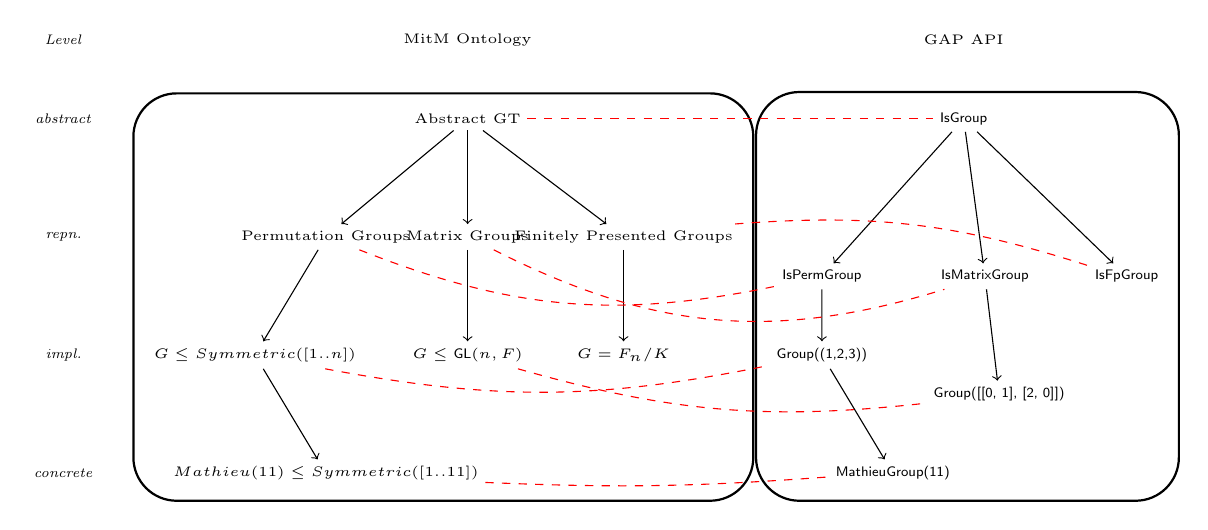
\begin{tikzpicture}[xscale=0.9]\tiny
\node (mitm) at (-2.7,8.5) {\emph{Level}}; 
\node (a) at (-2.7,7.5) {\emph{abstract}}; 
\node (b) at (-2.7,6) {\emph{repn.}}; 
\node (c) at (-2.7,4.5) {\emph{impl.}}; 
\node (d) at (-2.7,3) {\emph{concrete}}; 

\node (mitm) at (3,8.5) {MitM Ontology};

\node (grouptheory) at (3,7.5) {Abstract GT};
\node (permgrp) at (1,6) {\mylabel{Permutation Groups}};
\node (matgrp) at (3,6) {\mylabel{Matrix Groups}};
\node (finpresgrp) at (5.2,6) {\mylabel{Finitely Presented Groups}};
\draw[->] (grouptheory) -- (permgrp);
\draw[->] (grouptheory) -- (matgrp);
\draw[->] (grouptheory) -- (finpresgrp);

\node (symm) at (0,4.5) {$G\leq\text{Symmetric}([1..n])$};
\node (glnf) at (3,4.5) {$G\leq\textsf{GL}(n,F)$};
\node (fnk) at (5.2,4.5) {$G=F_n/K$};
\draw[->] (permgrp) -- (symm);
\draw[->] (matgrp) -- (glnf);
\draw[->] (finpresgrp) -- (fnk);

\node (mathieu) at (1,3) {$\text{Mathieu}(11)\leq\text{Symmetric}([1..11])$};
\draw[->] (symm) -- (mathieu);

 \node[draw,thick,fit=(grouptheory) (permgrp) (matgrp) (finpresgrp) (symm) (glnf) (fnk) (mathieu),
                   rounded corners=.55cm, inner sep=5pt] (mitmcloud) {};
                   
\node (gap) at (10,8.5) {GAP API};

\node (isgrp) at (10,7.5) {\textsf{IsGroup}};

\node (empty) at (10,3) {};
\node (ispermgrp) at (8,5.5) {\textsf{IsPermGroup}};
\node (ismatgrp) at (10.3,5.5) {\textsf{IsMatrixGroup}};
\node (isfpgrp) at (12.3,5.5) {\textsf{IsFpGroup}};
\draw[->] (isgrp) -- (ispermgrp);
\draw[->] (isgrp) -- (ismatgrp);
\draw[->] (isgrp) -- (isfpgrp);

\node (pgroup) at (8,4.5) { \textsf{Group((1,2,3))} };
\node (mgroup) at (10.5,4.0) { \textsf{Group([[0, 1], [2, 0]])} };
\node (cgroup) at (9,3)    { \textsf{MathieuGroup(11)} };

\draw[->] (ispermgrp) -- (pgroup);
\draw[->] (ismatgrp) -- (mgroup);
\draw[->] (pgroup) -- (cgroup);

 \node[draw,thick,fit=(isgrp) (ispermgrp) (ismatgrp) (isfpgrp) (empty) (pgroup) (mgroup) (cgroup),
                   rounded corners=.55cm, inner sep=5pt] (gapcloud) {};
                   
\draw[red,dashed] (grouptheory) -- (isgrp);
\draw[red,dashed] (permgrp) to[bend right=15] (ispermgrp);
\draw[red,dashed] (matgrp) to[bend right=20] (ismatgrp);
\draw[red,dashed] (finpresgrp) to[bend left=10] (isfpgrp);

\draw[red,dashed] (symm) to[bend right=10] (pgroup);
\draw[red,dashed] (glnf) to[bend right=10] (mgroup);
\draw[red,dashed] (mathieu) to[bend right=3] (cgroup);



%
%\node (Int) at (6,8.5) {Interfaces};
%
%\node (TT) at (4.9,3.5) {Type Theory};
%\node (ST) at (7.6,4.2) {Set Theory};
%\draw[<->,dotted] (TT) -- (ST);
%
%\node (Reals) at (4.7,4.8) {\textsf{Numbers}};
%\node (Nat) at (4.7,6) {$\mathbb N$};
%\draw[\arrowtipmono-\arrowtip] (Reals) -- (Nat);
%
%\node (FOrd) at (7.2,5.5) {Finite Ordinals};
%
%\node (PA) at (6,7) {Peano Axioms};
%\draw[<-] (FOrd) -- (PA);
%\draw[<-] (Nat) -- (PA);
%\draw[\arrowtipmono-\arrowtip] (ST) -- (FOrd);
%
% \node[draw,thick,fit=(ST) (Reals) (Nat) (FOrd) (PA) (TT),
%                   rounded corners=.55cm, inner sep=10pt] (PVScloud) {};
%
%\node (gap) at (11,8.5) {GAP API};
%
%\node (MNat) at (11,7) {\textsf{Nat}};
%\node (MOrd) at (11,3) {\textsf{Ordinals}};
%\draw[\arrowtipmono-\arrowtip] (MOrd) -- (MNat);
%
% \node[draw,thick,fit=(MNat) (MOrd),
%                   rounded corners=.55cm, inner sep=5pt] (PVScloud) {};
%
%\draw[red] (PVSfnd) -- (TT);
%\draw[red] (Mizfnd) -- (ST);
%\draw[red] (MOrd) -- (ST);
%\draw[red] (PVNat) -- (Nat);
%\draw[red] (PVnf) -- (Reals);
%\draw[red] (MNat) -- (FOrd);
%
%\draw[<->,dotted] (TT) -- (Reals);
%\draw[<->,dotted] (ST) -- (Reals);

\end{tikzpicture}
\end{document}

%%% Local Variables:
%%% mode: latex
%%% TeX-master: t
%%% End:

%  LocalWords:  providecommand mylabel tikzpicture mitm emph repn impl grouptheory matgrp
%  LocalWords:  permgrp finpresgrp symm leq glnf fnk draw,thick,fit mitmcloud isgrp FOrd
%  LocalWords:  ispermgrp ismatgrp isfpgrp gapcloud red,dashed mathbb arrowtipmono MNat
%  LocalWords:  arrowtip PVScloud MOrd PVSfnd Mizfnd PVnf

\medskip

At the abstract level, there is the theory of \emph{Groups}: the group axioms,
generating sets, homomorphisms, group actions, stabilisers, and orbits. This
also easily leads into definitions of centralisers\footnote{stabilisers of
elements under conjugation} and normalisers\footnote{stabilisers of subgroups under
conjugation}, stabiliser chains, Sylow-$p$ subgroups, Hall subroups, and many
other concepts. 

MMT also allows expressing that there are different equivalent definitions of a
concept: We defined group actions in two ways and used \emph{views} to express
their equivalence.

\smallskip

Abstract groups can be represented in many ways as concrete mathematical
objects suitable for computation: as groups of permutations, groups of matrices,
finitely presented groups, or using a polycyclic presentation.

Additionally, mathematicians often compute with canonical representatives of an
isomorphism class of groups: When a group theorist talks about the ``Dihedral
group of order 8'', they often have a particular representation in
mind, for example as a group that acts on the square by rotations
and reflections. In GAP this group would be represented as a group of
permutations, or by a polycyclic presentation.

Many representations arise naturally from \emph{group actions}: If we are
considering symmetry in a setting where we want to apply group theory, we start
with a group action.\ednote{MP@ALL: More concrete? More ``gripping''? I already
talked about the canonical example with the dihedral group}

The universal tool to bridge the gap between groups, representations and
canonical representatives are group homomorphisms, particularly isomorphisms,
which are used extensively in GAP. This is reflected in our approach.

\smallskip

At the lowest level there are implementation details: Permutation groups in GAP
are considered as finite subgroups of the group $S_{\mathbb{N}+}$, and defined by
providing a set of generating permutations. GAP then computes a stabiliser chain
for a group that was defined this way, and naturally considers the group to be a
subgroup of $S_{[1..n]}$, where $n$ is the largest point moved.

\smallskip

Building this part of the CGT MitM Ontology already posed a few challenges for
the MMT system, mostly to do with subtyping, since we needed to be able to talk
about all subgroups of a group, and all normal subgroups of a group. Quantifying
over these classes can lead to inconsistencies in the underlying type theory.
These challenges immediately translate into necessary
features in MMT, for example by introducing universe hierarchies.
\ednote{MP+FR+DM: Is this too gratuitous? Not concrete enough?}

\subsection{Alignments}

The initial alignments are currently produced by hand, but from some of the
initial alignments and the GAP API CDs we will be able to infer more alignments
automatically.

For example, the filter \texttt{IsGroup} is aligned with \texttt{Group}, and the
filter \texttt{IsPermGroup} is aligned with \texttt{Subgroup SymmetricGroup
  [1..n]}.
\ednote{MP: Need to be more concrete here, in particular we should maybe
  describe how GAP's notion of an action homomorphism translates through this?
  Also is this even correct?}

We formalised the theory of symmetric groups of a set; in GAP permutation groups
are represented as subgroups (with finite support) of the symmetric group of
$\mathbb{N}+$, and often one concretely has an isomorphism between the group one
is interested in and a subgroup of $S_{\mathbb{N}+}$, for example
via a group action.

\texttt{SylowSubgroup}s are more difficult: They are special groups in their
own right, namely groups whose size is a prime-power, but we also want them
to be identified with a certain subgroup of the group we are working
with.\ednote{MP: While I believe this to be an excellent additional example
  for MMT formalisation, this could be going too far for this paper}

\ednote{MP@ALL: We might want to be a bit careful/mention implementations of group
  theory for example in COQ where they did the Odd-Order-Proof?}
%%% Local Variables:
%%% mode: latex
%%% TeX-master: "paper"
%%% End:

%  LocalWords:  sec:cgt MueRoYuRa:abtafs17,MueGauKal:cacfms17 emph Sylow subroups medskip
%  LocalWords:  mathbb fig:cgtontology alignmentimg smallskip subtyping

\begin{figure}[ht]\centering\vspace*{-1em}
  \tikzinput{gap_singular_mitm_fig}
  \caption{MitM Interaction in Jane's Use Case}\label{fig:mitmpoc}\vspace*{-1em}
\end{figure}

Figure~\ref{fig:mitmpoc} shows the overall architecture with an MitM server as the central mediator.
All arrows represent the transfer of \OMMT objects via SCSCP.
Critically, the MitM server also maintains the alignments and uses them to convert between system dialects.

We have extended the \MMT system~\cite{Rabe:MAGMS13} with an SCSCP server/client so that it can receive/send objects from/to computation systems.
For the \GAP server, we built on pre-existing \SCSCP support.
To obtain an \SCSCP server for \Singular, which does not have native \SCSCP support, we wrapped \Singular in a python script that includes the \lstinline|pyscscp| library~\cite{py-scscp:on}.
In \Sage, we directly programmed the client interface to the MitM server. 

The resulting system forms the nucleus of the OpenDreamKit interoperability layer. It can already delegate computations between the three participating systems as long as the exchanged objects are covered by the MitM ontology, the alignments, and the formalizations of the system dialects.

\paragraph{Jane's Use Case} 
Initially, Jane has already built in \Sage the ring $R=\mathbb{Z}[X_1,X_2,X_3,X_4]$, the group $G=D_4$, the action $A$ of $G$ on $R$ that permutes the variables, and the polynomial $p = 3\cdot X_1 + 2\cdot X_2$.  She now calls
\begin{lstlisting}
  MitM.Singular(MitM.Gap.orbit(G, A, p)).Ideal().Groebner().sage()
\end{lstlisting}
which results in the following steps (the numbers on the edges of the
graph of Figure~\ref{fig:mitmpoc} indicate the order of communications when processing Jane's use case):
\begin{compactenum}
  \item Jane uses \Sage to call the MitM server with the command above, which includes both the computation to be performed and information about which system to use at which step.
  \item The MitM server translates \lstinline|MitM.Gap.orbit(G, A, p)| to the \GAP system dialect and sends it to \GAP.
  \item \GAP returns the orbit:
    \begin{displaymath}
      \begin{split}
        O = [3X_1 + 2X_2, 2X_3 + 3X_4, 3X_2 + 2X_3, 3X_3 + 2X_4,\\
        2X_2 + 3X_3, 3X_1 + 2X_4, 2X_1 + 3X_4, 2X_1 + 3X_2]\,.
      \end{split}
    \end{displaymath}
  \item The MitM server translates \lstinline|MitM.Singular(O).Ideal().Groebner()| to the \Singular system dialect and sends it to \Singular.
  \item \Singular returns the Gröbner base $B$.
  \item The MitM server translates $B$ to the \Sage system dialect and sends it to \Sage, where the result is shown to Jane.
    \begin{displaymath}
      B = [X_1 - X_4, X_2 - X_4, X_3 - X_4, 5X_4]\,.
    \end{displaymath}
  \end{compactenum}

\paragraph{Alternative Use Case}
Suppose Jon, one of Jane's colleagues, prefers working in \GAP, and he wants to
compute the Galois group of the rational polynomial $p = x^5 - 2$. He discovers
the \GAP package \texttt{radiroot}, which promises this functionality, but
unfortunately the package does not work for this polynomial and thus \GAP alone
cannot solve Jon's problem.

Jon hears from Jane that he should use \Sage, because she knows it can
compute Galois groups. So, from \GAP, he calls
\begin{lstlisting}
  G := MitM("Sage", "GaloisGroup",p)
\end{lstlisting}
which gives him the desired
Galois group as a \GAP permutation group. Having heard of Jane's
experiments, he can further run her orbit and Gröbner basis
calculation starting from this new group, without leaving his
favorite computing environment.
%\begin{lstinline}
%  G := MitM("Sage", "GaloisGroup",p)|

Finally, Jon, being a proficient \GAP user, also knows that he can now install a \defemph{method} in \GAP by calling 
\begin{lstlisting}
  InstallMethod(GaloisGroup, "for a polynomial", [IsUnivariatePolynomial], 
                p -> MitM("Sage", "GaloisGroup", p))
\end{lstlisting}
that will compute the Galois group of any rational polynomial transparently for him whenever he calls \lstinline|GaloisGroup| for a rational polynomial in \GAP. 
And thus (at the price of using multiple systems) a significant part of the 1800-line \lstinline|radiroot| package can be replaced by a few lines in GAP, taking advantage of the work of the \Sage community and participating in any future improvements of \Sage. 
In fact, Sage itself delegates to the PARI system -- another one of the OpenDreamKit systems -- for this computation.  So in the future \GAP might directly delegate to PARI instead, bypassing the need of iterated translations.

% $p =x^4-x^3-x^2+x+1$ over $\mathbb{Q}$ would have D_8 as galois group again...

%%% Local Variables:
%%% mode: latex
%%% TeX-master: "report"
%%% End:

%  LocalWords:  sec:case fig:mitmpoc IanJucKoh:sdm14,MathHub:on summarize sec:cgt pyscscp vspace lstlisting
%  LocalWords:  twiesing:msc17 centering tikzinput gap_singular_mitm_fig lstinline emph
%  LocalWords:  py-scscp:on oldpart mathbb cdot cdot Groebner Gröbner radiroot jist
%  LocalWords:  GaloisGroup galois

\section{Conclusion}\label{sec:concl}

We have shown how to extend the Math-in-the-Middle framework for integrating systems to mathematical data bases like the \lmfdb. 
The main idea is to embed knowledge sources as virtual theories, i.e. theories that are not -- theoretically or in practice -- limited in the number of declarations and allow dynamic loading and processing. 
For accessing real-world knowledge sources, we have developed the notion of codecs and integrated them into the MitM ontology framework. 
These codec's (and their MitM types) lift knowledge source access to the MitM level and thus enable object-level interoperability and allow humans (mathematicians) access using the concepts they are familiar with. 
Finally, we have shown a prototypical query translation facility that allows to delegate some of the processing to the underlying knowledge source and thus avoid thrashing of virtual theories. 

\paragraph{Related Work} Most other integration schemes employ a \textbf{homogenous approach}, where there is a master sytsem and all data is converted into that system. 
A paradigmatic example of this is the Wolfram Language and the Wolfram Alpha search engine~\cite{WolframAlpha:on}, which are based on the Mathematica kernel. 
This is very flexible for anyone owning a Matheamtica license and experienced in the Mathematica language and environment.

The MitM-based approach to interoperability of data sources and systems proposed in this paper is inherently a \textbf{heterogeneous approach}: systems and data sources are kept ``as is'', but their APIs are documented in a machine-actionable way that can be utilized for remote procedure calls, content format mediation, and service discovery. 
As a consequence, interaction between systems is very flexible.
For the data source integration via virtual theories presented in this paper this is important. 
For instance, we can just make an extension of \mmt or Sage which just act as a programmatic interface for e.g. \lmfdb. 

\paragraph{Future Work}
We have discussed the MitM+virtual theories methodology on the elliptic curves sub-base of the \lmfdb, which we have fully integrated. 
We are currently working on additional \lmfdb sub-bases. 
The main problem to be solved is to elicit the information for the respective schema theories from the \lmfdb community. 
Once that is accomplished, specifying them in the format discussed in this paper and writing the respective codecs is straightforward. 

Moreover, we are working on integrating the the Online Encyclopedia of Integer Sequences (OEIS~\cite{Sloane:OEIS,oeis}). 
Here we have a different problem: the OEIS database is essentially a flat ASCII file with different slots (for initial segments of the sequences, references, comments, and formulae); all minimally marked up ASCII art. 
In~\cite{LuzKoh:fsarfo16} we have already (heuristically) flexiformalized OEIS contents in \ommt; the next step will be to come up with codecs based on this basis and develop schema theories for OEIS.

\subsubsection*{Acknowledgements}
The authors gratefully acknowledge the fruitful discussions with other participants of
work package WP6, in particular John Cremona on the LMFDB and Dennis M\"uller on early
versions of the \ommt-based integration. We acknowledge financial support from the
OpenDreamKit Horizon 2020 European Research Infrastructures project (\#676541).

%%% Local Variables:
%%% mode: latex
%%% TeX-master: "paper"
%%% End:

%  LocalWords:  sec:concl subsubsection ommt lmfdb itemize Sloane:OEIS,oeis LuzKoh:fsarfo16 flexiformalized MitM-based textbf utilized
  
  
\printbibliography
\end{document}
%%% Local Variables:
%%% mode: latex
%%% TeX-master: t
%%% End:

%  LocalWords:  maketitle twb sec:intro DehKohKon:iop16 MueGauKal:cacfms17 optimized mitm
%  LocalWords:  itemize MitM-based sec:concl twiesing:msc17 printbibliography sec:mitm
%  LocalWords:  sec:mmt summarize sec:cgt sec:ift MueRoYuRa:abtafs17,MueGauKal:cacfms17
%  LocalWords:  cgt concl
